\section{Gesamtkonzept}
\label{sec:gesamtkonzept}

\textit{Silisloth} besteht aus drei Baugruppen: Aufhängung (A), Kontrollbox (B) und Greifmechanismus (C). Der Aufbau von \textit{Silisloth} ist in \imgrefplain{fig:laufkatze-links} (Ansicht links) und \imgrefplain{fig:laufkatze-rechts} (Ansicht rechts) als CAD-Modell ersichtlich.

In der Aufhängung wird das Antriebsrad von einem Getriebemotor (1) mit einer 1:1-Übersetzung angetrieben. Das Seil wird an den beiden Laufrädern (2, 3) und am Antriebsrad (4) umgelenkt. Die Kontrollbox ist mit einem Bolzen gelenkig mit der Aufhängung gelagert, damit der Greifer immer horizontal liegt. Der Greifmechanismus wird mit einem Flaschenzug (5) auf und ab bewegt. Das Seil für den Flaschenzug wird durch eine 3-Punkt-Umlenkung an einer Seiltrommel (6) aufgewickelt. Diese wird durch einen Stepper-Motor (7) mit einer Übersetzung von 1:2 angetrieben. Die Luftzufuhr für den Silikongreifer (8) erfolgt durch die Luftpumpe (9) und wird über das magnetische Ventil (10) geregelt.

Die Ultraschallsensoren (11, 12) sind so positioniert, dass keine Komponente von \textit{Silisloth} während der Fahrt die Messdaten der Sensoren verfälschen könnte. Der erste Ultraschallsensor (11) misst die Distanz zum Boden, der zweite Ultraschallsensor (12) die Distanz zum Endmast.

Das Entwicklerboard (13) ist auf der rechten Seite angebracht. Die Akkus (14) und der Mikrocontroller (15) befinden sich im Inneren des Gehäuses. Vorne ist eine Kamera (16) angebracht.

\begin{figure}
    \centering
    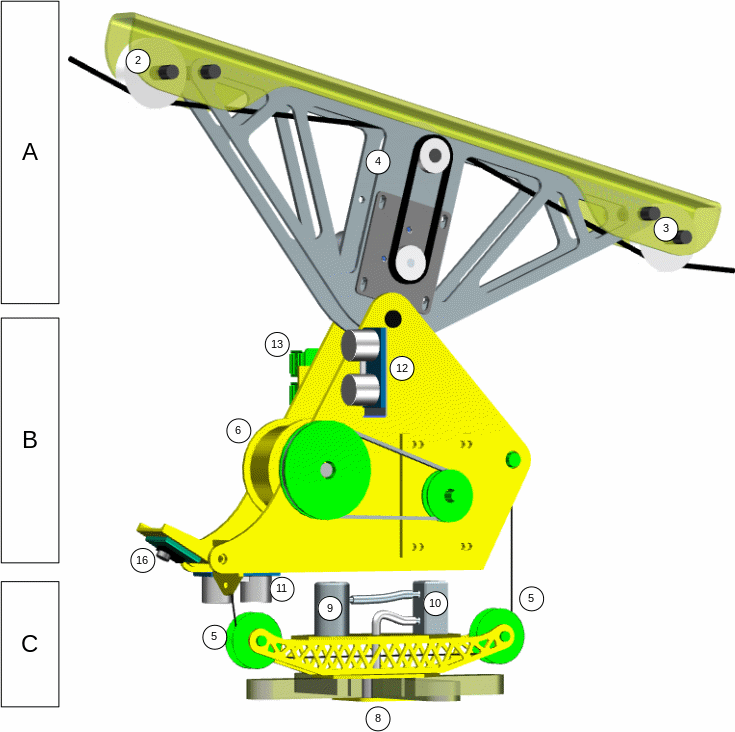
\includegraphics[width=\linewidth]{pics/cad-links.png}
    \caption{CAD-Modell von \textit{Silisloth} (Ansicht links)}
    \label{fig:laufkatze-links}
\end{figure}

\begin{figure}
    \centering
    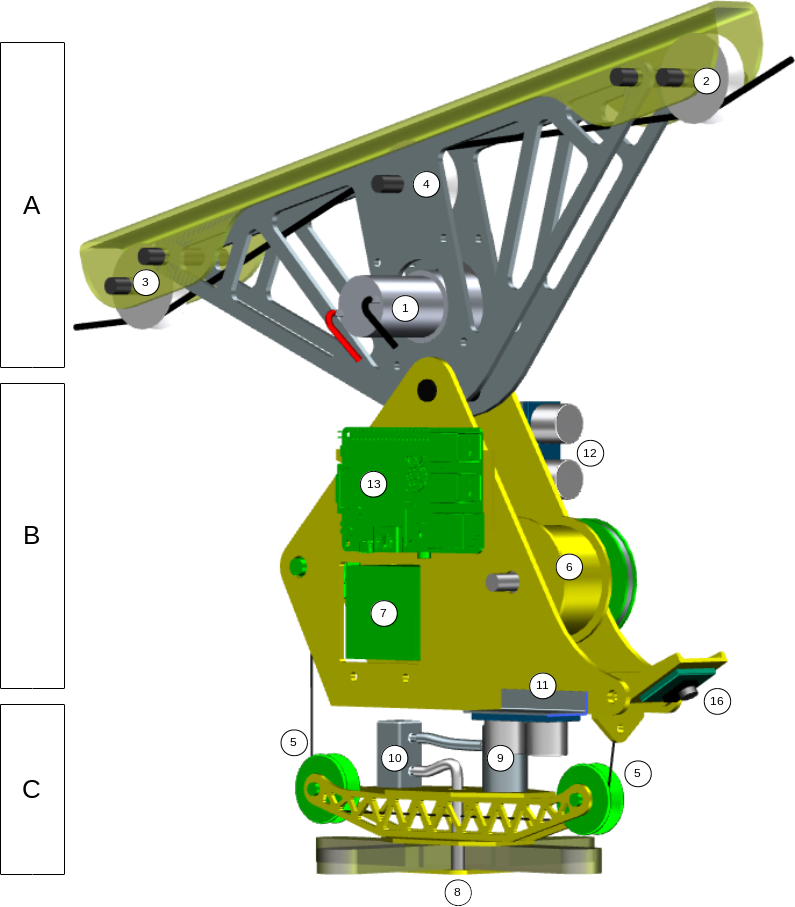
\includegraphics[width=\linewidth]{pics/cad-rechts.png}
    \caption{CAD-Modell von \textit{Silisloth} (Ansicht rechts)}
    \label{fig:laufkatze-rechts}
\end{figure}

